% Options for packages loaded elsewhere
\PassOptionsToPackage{unicode}{hyperref}
\PassOptionsToPackage{hyphens}{url}
%
\documentclass[
]{article}
\usepackage{amsmath,amssymb}
\usepackage{lmodern}
\usepackage{ifxetex,ifluatex}
\ifnum 0\ifxetex 1\fi\ifluatex 1\fi=0 % if pdftex
  \usepackage[T1]{fontenc}
  \usepackage[utf8]{inputenc}
  \usepackage{textcomp} % provide euro and other symbols
\else % if luatex or xetex
  \usepackage{unicode-math}
  \defaultfontfeatures{Scale=MatchLowercase}
  \defaultfontfeatures[\rmfamily]{Ligatures=TeX,Scale=1}
\fi
% Use upquote if available, for straight quotes in verbatim environments
\IfFileExists{upquote.sty}{\usepackage{upquote}}{}
\IfFileExists{microtype.sty}{% use microtype if available
  \usepackage[]{microtype}
  \UseMicrotypeSet[protrusion]{basicmath} % disable protrusion for tt fonts
}{}
\makeatletter
\@ifundefined{KOMAClassName}{% if non-KOMA class
  \IfFileExists{parskip.sty}{%
    \usepackage{parskip}
  }{% else
    \setlength{\parindent}{0pt}
    \setlength{\parskip}{6pt plus 2pt minus 1pt}}
}{% if KOMA class
  \KOMAoptions{parskip=half}}
\makeatother
\usepackage{xcolor}
\IfFileExists{xurl.sty}{\usepackage{xurl}}{} % add URL line breaks if available
\IfFileExists{bookmark.sty}{\usepackage{bookmark}}{\usepackage{hyperref}}
\hypersetup{
  pdftitle={MATH 629 HW 4 Solutions},
  pdfauthor={Drew Lazar},
  hidelinks,
  pdfcreator={LaTeX via pandoc}}
\urlstyle{same} % disable monospaced font for URLs
\usepackage[margin=1in]{geometry}
\usepackage{color}
\usepackage{fancyvrb}
\newcommand{\VerbBar}{|}
\newcommand{\VERB}{\Verb[commandchars=\\\{\}]}
\DefineVerbatimEnvironment{Highlighting}{Verbatim}{commandchars=\\\{\}}
% Add ',fontsize=\small' for more characters per line
\usepackage{framed}
\definecolor{shadecolor}{RGB}{248,248,248}
\newenvironment{Shaded}{\begin{snugshade}}{\end{snugshade}}
\newcommand{\AlertTok}[1]{\textcolor[rgb]{0.94,0.16,0.16}{#1}}
\newcommand{\AnnotationTok}[1]{\textcolor[rgb]{0.56,0.35,0.01}{\textbf{\textit{#1}}}}
\newcommand{\AttributeTok}[1]{\textcolor[rgb]{0.77,0.63,0.00}{#1}}
\newcommand{\BaseNTok}[1]{\textcolor[rgb]{0.00,0.00,0.81}{#1}}
\newcommand{\BuiltInTok}[1]{#1}
\newcommand{\CharTok}[1]{\textcolor[rgb]{0.31,0.60,0.02}{#1}}
\newcommand{\CommentTok}[1]{\textcolor[rgb]{0.56,0.35,0.01}{\textit{#1}}}
\newcommand{\CommentVarTok}[1]{\textcolor[rgb]{0.56,0.35,0.01}{\textbf{\textit{#1}}}}
\newcommand{\ConstantTok}[1]{\textcolor[rgb]{0.00,0.00,0.00}{#1}}
\newcommand{\ControlFlowTok}[1]{\textcolor[rgb]{0.13,0.29,0.53}{\textbf{#1}}}
\newcommand{\DataTypeTok}[1]{\textcolor[rgb]{0.13,0.29,0.53}{#1}}
\newcommand{\DecValTok}[1]{\textcolor[rgb]{0.00,0.00,0.81}{#1}}
\newcommand{\DocumentationTok}[1]{\textcolor[rgb]{0.56,0.35,0.01}{\textbf{\textit{#1}}}}
\newcommand{\ErrorTok}[1]{\textcolor[rgb]{0.64,0.00,0.00}{\textbf{#1}}}
\newcommand{\ExtensionTok}[1]{#1}
\newcommand{\FloatTok}[1]{\textcolor[rgb]{0.00,0.00,0.81}{#1}}
\newcommand{\FunctionTok}[1]{\textcolor[rgb]{0.00,0.00,0.00}{#1}}
\newcommand{\ImportTok}[1]{#1}
\newcommand{\InformationTok}[1]{\textcolor[rgb]{0.56,0.35,0.01}{\textbf{\textit{#1}}}}
\newcommand{\KeywordTok}[1]{\textcolor[rgb]{0.13,0.29,0.53}{\textbf{#1}}}
\newcommand{\NormalTok}[1]{#1}
\newcommand{\OperatorTok}[1]{\textcolor[rgb]{0.81,0.36,0.00}{\textbf{#1}}}
\newcommand{\OtherTok}[1]{\textcolor[rgb]{0.56,0.35,0.01}{#1}}
\newcommand{\PreprocessorTok}[1]{\textcolor[rgb]{0.56,0.35,0.01}{\textit{#1}}}
\newcommand{\RegionMarkerTok}[1]{#1}
\newcommand{\SpecialCharTok}[1]{\textcolor[rgb]{0.00,0.00,0.00}{#1}}
\newcommand{\SpecialStringTok}[1]{\textcolor[rgb]{0.31,0.60,0.02}{#1}}
\newcommand{\StringTok}[1]{\textcolor[rgb]{0.31,0.60,0.02}{#1}}
\newcommand{\VariableTok}[1]{\textcolor[rgb]{0.00,0.00,0.00}{#1}}
\newcommand{\VerbatimStringTok}[1]{\textcolor[rgb]{0.31,0.60,0.02}{#1}}
\newcommand{\WarningTok}[1]{\textcolor[rgb]{0.56,0.35,0.01}{\textbf{\textit{#1}}}}
\usepackage{graphicx}
\makeatletter
\def\maxwidth{\ifdim\Gin@nat@width>\linewidth\linewidth\else\Gin@nat@width\fi}
\def\maxheight{\ifdim\Gin@nat@height>\textheight\textheight\else\Gin@nat@height\fi}
\makeatother
% Scale images if necessary, so that they will not overflow the page
% margins by default, and it is still possible to overwrite the defaults
% using explicit options in \includegraphics[width, height, ...]{}
\setkeys{Gin}{width=\maxwidth,height=\maxheight,keepaspectratio}
% Set default figure placement to htbp
\makeatletter
\def\fps@figure{htbp}
\makeatother
\setlength{\emergencystretch}{3em} % prevent overfull lines
\providecommand{\tightlist}{%
  \setlength{\itemsep}{0pt}\setlength{\parskip}{0pt}}
\setcounter{secnumdepth}{-\maxdimen} % remove section numbering
\ifluatex
  \usepackage{selnolig}  % disable illegal ligatures
\fi

\title{MATH 629 HW 4 Solutions}
\author{Drew Lazar}
\date{}

\begin{document}
\maketitle

\hypertarget{cleaning-up-and-loading-necessary-packages}{%
\subsection{Cleaning up and loading necessary
packages}\label{cleaning-up-and-loading-necessary-packages}}

\begin{Shaded}
\begin{Highlighting}[]
\FunctionTok{rm}\NormalTok{(}\AttributeTok{list=}\FunctionTok{ls}\NormalTok{())}
\FunctionTok{library}\NormalTok{(survival)}
\FunctionTok{library}\NormalTok{(dplyr)}
\end{Highlighting}
\end{Shaded}

\begin{verbatim}
## 
## Attaching package: 'dplyr'
\end{verbatim}

\begin{verbatim}
## The following objects are masked from 'package:stats':
## 
##     filter, lag
\end{verbatim}

\begin{verbatim}
## The following objects are masked from 'package:base':
## 
##     intersect, setdiff, setequal, union
\end{verbatim}

\hypertarget{loading-the-data}{%
\subsection{1 loading the data}\label{loading-the-data}}

\begin{Shaded}
\begin{Highlighting}[]
\NormalTok{Ven.reset }\OtherTok{\textless{}{-}}\FunctionTok{read.csv}\NormalTok{(}\StringTok{"VenresetMft.csv"}\NormalTok{, }\AttributeTok{header =} \ConstantTok{TRUE}\NormalTok{)}
\end{Highlighting}
\end{Shaded}

\#\#2 Test the PH assumption \#\#2i. GOF using Schoenfeld Residuals

\begin{Shaded}
\begin{Highlighting}[]
\NormalTok{Y}\OtherTok{\textless{}{-}}\FunctionTok{Surv}\NormalTok{(Ven.reset}\SpecialCharTok{$}\NormalTok{eventtime,Ven.reset}\SpecialCharTok{$}\NormalTok{status)}
\NormalTok{Coxph.addicts}\OtherTok{=}\FunctionTok{coxph}\NormalTok{(Y}\SpecialCharTok{\textasciitilde{}}\NormalTok{Setting}\SpecialCharTok{+}\NormalTok{LO2}\SpecialCharTok{+}\NormalTok{Mft,}\AttributeTok{data=}\NormalTok{Ven.reset)}
\FunctionTok{summary}\NormalTok{(Coxph.addicts)}
\end{Highlighting}
\end{Shaded}

\begin{verbatim}
## Call:
## coxph(formula = Y ~ Setting + LO2 + Mft, data = Ven.reset)
## 
##   n= 150, number of events= 145 
## 
##             coef exp(coef) se(coef)      z Pr(>|z|)    
## Setting  0.99883   2.71509  0.12190  8.194 2.52e-16 ***
## LO2      0.92339   2.51781  0.07785 11.861  < 2e-16 ***
## Mft     -0.26092   0.77034  0.18002 -1.449    0.147    
## ---
## Signif. codes:  0 '***' 0.001 '**' 0.01 '*' 0.05 '.' 0.1 ' ' 1
## 
##         exp(coef) exp(-coef) lower .95 upper .95
## Setting    2.7151     0.3683    2.1381     3.448
## LO2        2.5178     0.3972    2.1615     2.933
## Mft        0.7703     1.2981    0.5413     1.096
## 
## Concordance= 0.833  (se = 0.013 )
## Likelihood ratio test= 193.7  on 3 df,   p=<2e-16
## Wald test            = 160  on 3 df,   p=<2e-16
## Score (logrank) test = 175.9  on 3 df,   p=<2e-16
\end{verbatim}

\begin{Shaded}
\begin{Highlighting}[]
\FunctionTok{cox.zph}\NormalTok{(Coxph.addicts,}\AttributeTok{transform=}\NormalTok{rank)}
\end{Highlighting}
\end{Shaded}

\begin{verbatim}
##            chisq df      p
## Setting 1.92e+00  1 0.1658
## LO2     5.82e-04  1 0.9808
## Mft     9.87e+00  1 0.0017
## GLOBAL  1.60e+01  3 0.0011
\end{verbatim}

\#\#2ii. Testing MFt with Setting and LO2 in the model

\begin{Shaded}
\begin{Highlighting}[]
\CommentTok{\#Stratify Ventilator Data set by TR}
\NormalTok{Ven.reset0}\OtherTok{\textless{}{-}}\NormalTok{Ven.reset[Ven.reset}\SpecialCharTok{$}\NormalTok{Mft}\SpecialCharTok{==}\DecValTok{0}\NormalTok{, ]}
\NormalTok{Ven.reset1}\OtherTok{\textless{}{-}}\NormalTok{Ven.reset[Ven.reset}\SpecialCharTok{$}\NormalTok{Mft}\SpecialCharTok{==}\DecValTok{1}\NormalTok{, ]}
\CommentTok{\#Create Survival Objects for both strata }
\NormalTok{Y0}\OtherTok{\textless{}{-}}\FunctionTok{Surv}\NormalTok{(Ven.reset0}\SpecialCharTok{$}\NormalTok{eventtime,Ven.reset0}\SpecialCharTok{$}\NormalTok{status}\SpecialCharTok{==}\DecValTok{1}\NormalTok{)}
\NormalTok{Y1}\OtherTok{\textless{}{-}}\FunctionTok{Surv}\NormalTok{(Ven.reset1}\SpecialCharTok{$}\NormalTok{eventtime,Ven.reset1}\SpecialCharTok{$}\NormalTok{status}\SpecialCharTok{==}\DecValTok{1}\NormalTok{)}
\CommentTok{\#Fit Cox PH models to both strata}
\NormalTok{Coxph.Ven.m0}\OtherTok{=}\FunctionTok{coxph}\NormalTok{(Y0}\SpecialCharTok{\textasciitilde{}}\NormalTok{LO2}\SpecialCharTok{+}\NormalTok{Setting,}\AttributeTok{data=}\NormalTok{Ven.reset0)}
\NormalTok{Coxph.Ven.m1}\OtherTok{=}\FunctionTok{coxph}\NormalTok{(Y1}\SpecialCharTok{\textasciitilde{}}\NormalTok{LO2}\SpecialCharTok{+}\NormalTok{Setting,}\AttributeTok{data=}\NormalTok{Ven.reset1)}
\CommentTok{\#get the overall mean of LO2 and Setting }
\NormalTok{meanLO2}\OtherTok{=}\FunctionTok{mean}\NormalTok{(Ven.reset}\SpecialCharTok{$}\NormalTok{LO2)}
\NormalTok{meanSetting}\OtherTok{=}\FunctionTok{mean}\NormalTok{(Ven.reset}\SpecialCharTok{$}\NormalTok{Setting)}
\CommentTok{\#plot our adjusted survival curves }
\NormalTok{pattern}\OtherTok{=}\FunctionTok{data.frame}\NormalTok{(}\AttributeTok{LO2=}\NormalTok{meanLO2,}\AttributeTok{Setting=}\NormalTok{meanSetting)}
\FunctionTok{plot}\NormalTok{(}\FunctionTok{survfit}\NormalTok{(Coxph.Ven.m0,}\AttributeTok{newdata=}\NormalTok{pattern),}\AttributeTok{fun=}\StringTok{"cloglog"}\NormalTok{,}\AttributeTok{conf.int=}\NormalTok{F,}\AttributeTok{xlim=}\FunctionTok{c}\NormalTok{(}\DecValTok{1}\NormalTok{,}\DecValTok{23}\NormalTok{),}\AttributeTok{ylim=}\FunctionTok{c}\NormalTok{(}\SpecialCharTok{{-}}\FloatTok{3.9}\NormalTok{,}\FloatTok{2.3}\NormalTok{),}\AttributeTok{main=}\StringTok{"Adjusted log{-}log for Mft=0 vs Mft=1"}\NormalTok{,}\AttributeTok{col=}\FunctionTok{c}\NormalTok{(}\StringTok{\textquotesingle{}blue\textquotesingle{}}\NormalTok{))}
\FunctionTok{par}\NormalTok{(}\AttributeTok{new=}\ConstantTok{TRUE}\NormalTok{)}
\FunctionTok{plot}\NormalTok{(}\FunctionTok{survfit}\NormalTok{(Coxph.Ven.m1,}\AttributeTok{newdata=}\NormalTok{pattern),}\AttributeTok{fun=}\StringTok{"cloglog"}\NormalTok{,}\AttributeTok{conf.int=}\NormalTok{F,}\AttributeTok{xlim=}\FunctionTok{c}\NormalTok{(}\DecValTok{1}\NormalTok{,}\DecValTok{23}\NormalTok{),}\AttributeTok{ylim=}\FunctionTok{c}\NormalTok{(}\SpecialCharTok{{-}}\FloatTok{3.9}\NormalTok{,}\FloatTok{2.3}\NormalTok{),}\AttributeTok{col=}\FunctionTok{c}\NormalTok{(}\StringTok{\textquotesingle{}red\textquotesingle{}}\NormalTok{))}
\FunctionTok{legend}\NormalTok{(}\StringTok{"bottomright"}\NormalTok{,}\AttributeTok{cex=}\FloatTok{1.5}\NormalTok{,}\FunctionTok{c}\NormalTok{(}\StringTok{"Mft=0"}\NormalTok{,}\StringTok{"Mft=1"}\NormalTok{),}\AttributeTok{lty=}\FunctionTok{c}\NormalTok{(}\StringTok{"solid"}\NormalTok{),}\AttributeTok{col=}\FunctionTok{c}\NormalTok{(}\StringTok{"blue"}\NormalTok{,}\StringTok{"red"}\NormalTok{))}
\end{Highlighting}
\end{Shaded}

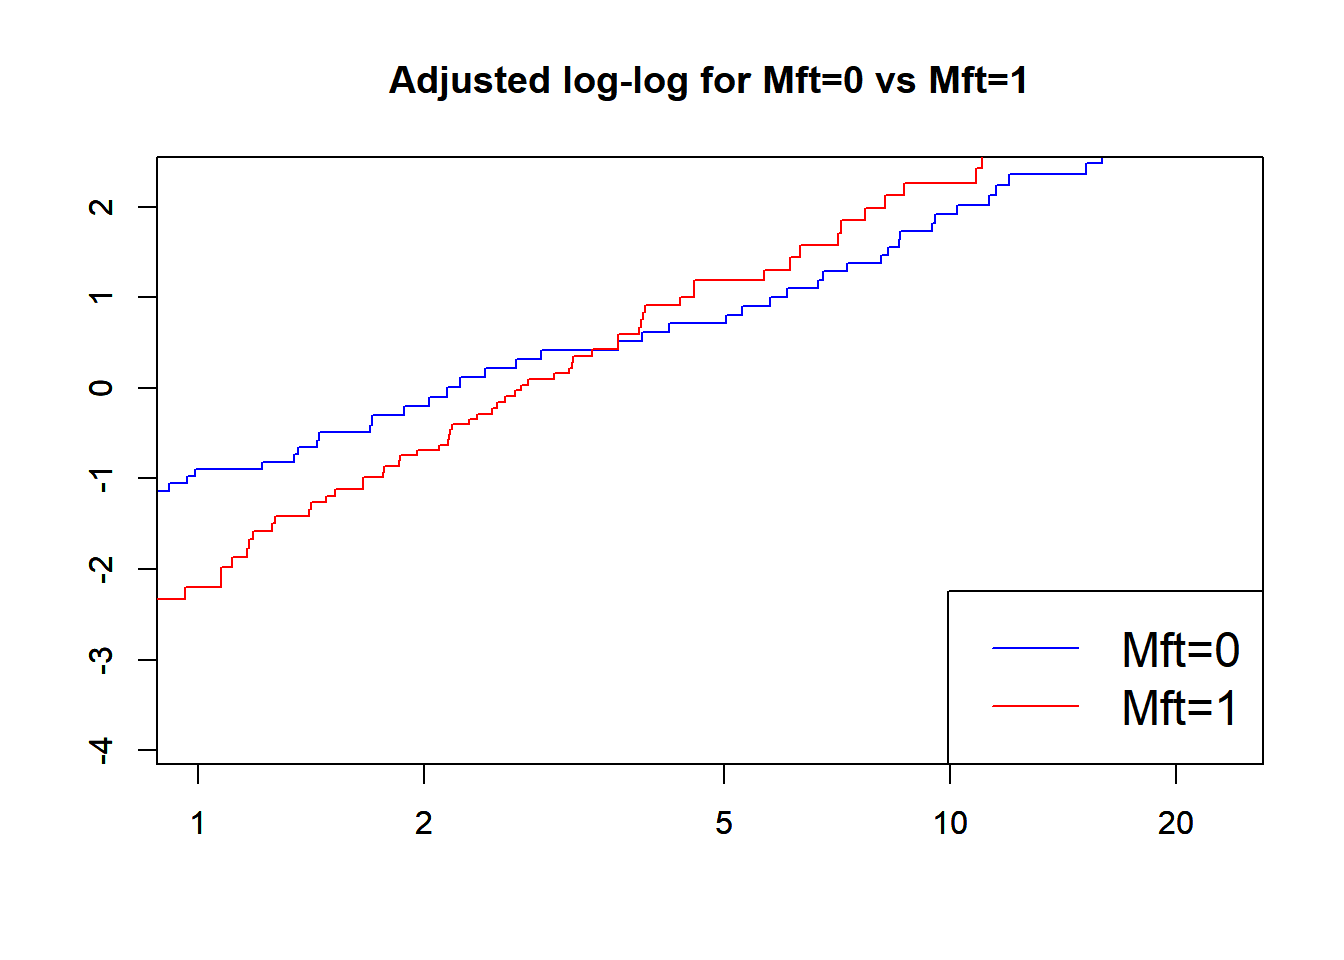
\includegraphics{HW4_629Solutions_files/figure-latex/unnamed-chunk-5-1.pdf}

\textbf{The Schoenfeld Residuals for Setting, LO2 and Mft are 0.1658,
0.9808 and 0.0017, respectively. Also, the adjusted log-log plots for
Mft clearly cross and are not parallel throughout the study. Both of
these suggests that Mft doesn't satisfy the PH assumption with Setting
and LO2 in the model. }

\hypertarget{stratification-by-mft}{%
\subsection{3. Stratification by Mft}\label{stratification-by-mft}}

\hypertarget{i.-fit-a-stratified-model-without-interaction.}{%
\subsection{3i. Fit a stratified model without
interaction.}\label{i.-fit-a-stratified-model-without-interaction.}}

\begin{Shaded}
\begin{Highlighting}[]
\CommentTok{\#i Fit a stratified model }
\NormalTok{Y}\OtherTok{\textless{}{-}}\FunctionTok{Surv}\NormalTok{(Ven.reset}\SpecialCharTok{$}\NormalTok{eventtime,Ven.reset}\SpecialCharTok{$}\NormalTok{status}\SpecialCharTok{==}\DecValTok{1}\NormalTok{)}
\NormalTok{coxph.Ven.m1}\OtherTok{\textless{}{-}}\FunctionTok{coxph}\NormalTok{(Y}\SpecialCharTok{\textasciitilde{}}\NormalTok{Setting }\SpecialCharTok{+}\NormalTok{ LO2 }\SpecialCharTok{+} \FunctionTok{strata}\NormalTok{(Mft),}\AttributeTok{data=}\NormalTok{Ven.reset)}
\FunctionTok{summary}\NormalTok{(coxph.Ven.m1)}
\end{Highlighting}
\end{Shaded}

\begin{verbatim}
## Call:
## coxph(formula = Y ~ Setting + LO2 + strata(Mft), data = Ven.reset)
## 
##   n= 150, number of events= 145 
## 
##            coef exp(coef) se(coef)      z Pr(>|z|)    
## Setting 0.93998   2.55992  0.12496  7.522 5.38e-14 ***
## LO2     0.84471   2.32729  0.07902 10.689  < 2e-16 ***
## ---
## Signif. codes:  0 '***' 0.001 '**' 0.01 '*' 0.05 '.' 0.1 ' ' 1
## 
##         exp(coef) exp(-coef) lower .95 upper .95
## Setting     2.560     0.3906     2.004     3.270
## LO2         2.327     0.4297     1.993     2.717
## 
## Concordance= 0.801  (se = 0.018 )
## Likelihood ratio test= 163.7  on 2 df,   p=<2e-16
## Wald test            = 128.3  on 2 df,   p=<2e-16
## Score (logrank) test = 147.9  on 2 df,   p=<2e-16
\end{verbatim}

Our fitted stratified Cox PH model is:
\(h_g(X,t)=h_{g0}(t)\exp(0.96368X_1+0.83814X_2)\) for \(g=1,2\) with
\(X_1=Setting\) and \(X_2=LO2\).

\hypertarget{ii.-wald-test-to-test-for-significance-of-setting-and-lo2}{%
\subsection{3ii. Wald test to test for significance of Setting and
LO2}\label{ii.-wald-test-to-test-for-significance-of-setting-and-lo2}}

Both setting an LO2 have very small p-values ( 5.14e-14 and
\textless2e-16, respectively) and thus are significant at
\(\alpha=0.05\).

\hypertarget{iii.-likelihood-ratio-test-to-test-for-overall-significance-of-setting-and-lo2.}{%
\subsection{3iii. Likelihood ratio test to test for overall significance
of Setting and
LO2.}\label{iii.-likelihood-ratio-test-to-test-for-overall-significance-of-setting-and-lo2.}}

\begin{Shaded}
\begin{Highlighting}[]
\NormalTok{coxph.Ven.m1}\SpecialCharTok{$}\NormalTok{loglik}
\end{Highlighting}
\end{Shaded}

\begin{verbatim}
## [1] -500.7220 -418.8862
\end{verbatim}

\begin{Shaded}
\begin{Highlighting}[]
\NormalTok{CSstat }\OtherTok{=} \SpecialCharTok{{-}}\DecValTok{2}\SpecialCharTok{*}\NormalTok{(coxph.Ven.m1}\SpecialCharTok{$}\NormalTok{loglik[}\DecValTok{1}\NormalTok{]}\SpecialCharTok{{-}}\NormalTok{coxph.Ven.m1}\SpecialCharTok{$}\NormalTok{loglik[}\DecValTok{2}\NormalTok{])}
\FunctionTok{print}\NormalTok{(}\FunctionTok{paste}\NormalTok{(}\StringTok{"The value of our test statistic is"}\NormalTok{, CSstat))}
\end{Highlighting}
\end{Shaded}

\begin{verbatim}
## [1] "The value of our test statistic is 163.671623032107"
\end{verbatim}

\begin{Shaded}
\begin{Highlighting}[]
\NormalTok{CV }\OtherTok{=} \FunctionTok{qchisq}\NormalTok{(.}\DecValTok{95}\NormalTok{,}\AttributeTok{df=}\DecValTok{2}\NormalTok{)}
\FunctionTok{print}\NormalTok{(}\FunctionTok{paste}\NormalTok{(}\StringTok{"Our critical value is:"}\NormalTok{,CV))}
\end{Highlighting}
\end{Shaded}

\begin{verbatim}
## [1] "Our critical value is: 5.99146454710798"
\end{verbatim}

\begin{Shaded}
\begin{Highlighting}[]
\NormalTok{CSstat}\SpecialCharTok{\textgreater{}}\NormalTok{CV}
\end{Highlighting}
\end{Shaded}

\begin{verbatim}
## [1] TRUE
\end{verbatim}

\begin{Shaded}
\begin{Highlighting}[]
\NormalTok{pvalue1}\OtherTok{=}\FunctionTok{pchisq}\NormalTok{(CSstat,}\AttributeTok{df =} \DecValTok{2}\NormalTok{,}\AttributeTok{lower.tail =} \ConstantTok{FALSE}\NormalTok{)}
\FunctionTok{print}\NormalTok{(}\FunctionTok{paste}\NormalTok{(}\StringTok{"Our p value is:"}\NormalTok{,pvalue1))}
\end{Highlighting}
\end{Shaded}

\begin{verbatim}
## [1] "Our p value is: 2.87844964568391e-36"
\end{verbatim}

Our test statistic has a value of 163.6716 and our critical value is
5.9915. As 163.6716\textgreater5.9915 we reject
\(H_0: \beta_1=\beta_2=0\) in
\(h_g(X,t)=h_{g0}(t)\exp(\beta_1 X_1+ \beta_2 X_2)\).

\hypertarget{iv.}{%
\subsection{3iv.}\label{iv.}}

For every unit increase in Setting the hazard increases by a factor of
\(e^{0.93998}=2.560\) and for every unit increase in LO2 the hazard
increases by a factor of \(e^{0.84471}=2.327\).

\hypertarget{iv.-plotting-adjusted-survival-curves}{%
\subsection{3iv. Plotting adjusted Survival
Curves}\label{iv.-plotting-adjusted-survival-curves}}

\begin{Shaded}
\begin{Highlighting}[]
\NormalTok{meanLO2}\OtherTok{=}\FunctionTok{mean}\NormalTok{(Ven.reset}\SpecialCharTok{$}\NormalTok{LO2)}
\NormalTok{pattern1}\OtherTok{=}\FunctionTok{data.frame}\NormalTok{(}\AttributeTok{Setting=}\DecValTok{0}\NormalTok{,}\AttributeTok{LO2=}\NormalTok{meanLO2)}
\FunctionTok{plot}\NormalTok{(}\FunctionTok{survfit}\NormalTok{(coxph.Ven.m1,}\AttributeTok{newdata=}\NormalTok{pattern1),}\AttributeTok{col=}\FunctionTok{c}\NormalTok{(}\StringTok{\textquotesingle{}blue\textquotesingle{}}\NormalTok{,}\StringTok{\textquotesingle{}red\textquotesingle{}}\NormalTok{),}\AttributeTok{conf.int=}\NormalTok{F,}\AttributeTok{main=}\StringTok{"Adjusted survival for Setting=0, 1 and 2, mean(LO2) from stratified Cox PH model"}\NormalTok{)}
\NormalTok{pattern2}\OtherTok{=}\FunctionTok{data.frame}\NormalTok{(}\AttributeTok{Setting=}\DecValTok{1}\NormalTok{,}\AttributeTok{LO2=}\NormalTok{meanLO2)}
\FunctionTok{par}\NormalTok{(}\AttributeTok{new=}\ConstantTok{TRUE}\NormalTok{)}
\FunctionTok{plot}\NormalTok{(}\FunctionTok{survfit}\NormalTok{(coxph.Ven.m1,}\AttributeTok{newdata=}\NormalTok{pattern2),}\AttributeTok{col=}\FunctionTok{c}\NormalTok{(}\StringTok{\textquotesingle{}blue\textquotesingle{}}\NormalTok{,}\StringTok{\textquotesingle{}red\textquotesingle{}}\NormalTok{), }\AttributeTok{lty=}\FunctionTok{c}\NormalTok{(}\StringTok{\textquotesingle{}dashed\textquotesingle{}}\NormalTok{),}\AttributeTok{conf.int=}\NormalTok{F)}
\NormalTok{pattern3}\OtherTok{=}\FunctionTok{data.frame}\NormalTok{(}\AttributeTok{Setting=}\DecValTok{2}\NormalTok{,}\AttributeTok{LO2=}\NormalTok{meanLO2)}
\FunctionTok{par}\NormalTok{(}\AttributeTok{new=}\ConstantTok{TRUE}\NormalTok{)}
\FunctionTok{plot}\NormalTok{(}\FunctionTok{survfit}\NormalTok{(coxph.Ven.m1,}\AttributeTok{newdata=}\NormalTok{pattern3),}\AttributeTok{col=}\FunctionTok{c}\NormalTok{(}\StringTok{\textquotesingle{}blue\textquotesingle{}}\NormalTok{,}\StringTok{\textquotesingle{}red\textquotesingle{}}\NormalTok{), }\AttributeTok{lty=}\FunctionTok{c}\NormalTok{(}\StringTok{\textquotesingle{}dotted\textquotesingle{}}\NormalTok{),}\AttributeTok{conf.int=}\NormalTok{F)}
\FunctionTok{legend}\NormalTok{(}\StringTok{"topright"}\NormalTok{,}\AttributeTok{cex=}\FloatTok{1.5}\NormalTok{,}\FunctionTok{c}\NormalTok{(}\StringTok{"Setting=0, Mft=0"}\NormalTok{,}\StringTok{"Setting=0, Mft=1"}\NormalTok{,}\StringTok{"Setting=1, Mft=0"}\NormalTok{,}\StringTok{"Setting=1,Mft=1"}\NormalTok{,}\StringTok{"Setting=2, Mft=0"}\NormalTok{,}\StringTok{"Setting=2, Mft=1"}\NormalTok{),}\AttributeTok{lty=}\FunctionTok{c}\NormalTok{(}\StringTok{"solid"}\NormalTok{,}\StringTok{"solid"}\NormalTok{,}\StringTok{"dashed"}\NormalTok{,}\StringTok{"dashed"}\NormalTok{,}\StringTok{"dotted"}\NormalTok{,}\StringTok{"dotted"}\NormalTok{),}\AttributeTok{col=}\FunctionTok{c}\NormalTok{(}\StringTok{"blue"}\NormalTok{,}\StringTok{"red"}\NormalTok{))}
\end{Highlighting}
\end{Shaded}

\includegraphics{HW4_629Solutions_files/figure-latex/unnamed-chunk-8-1.pdf}
The curves do not suggest significant interaction between Setting and
Mft adjusted for LO2. The changes in Survival experience from Setting=0
to Setting=1 to Setting=2 looks quite similar for Mft=0 and Mft=1.

\hypertarget{fitting-and-examining-a-stratified-cox-ph-model-with-interaction}{%
\subsection{4. Fitting and examining a stratified Cox PH model with
interaction}\label{fitting-and-examining-a-stratified-cox-ph-model-with-interaction}}

\hypertarget{i.}{%
\subsection{4i.}\label{i.}}

\begin{Shaded}
\begin{Highlighting}[]
\NormalTok{coxph.Ven.int.m1}\OtherTok{\textless{}{-}}\FunctionTok{coxph}\NormalTok{(Y}\SpecialCharTok{\textasciitilde{}}\NormalTok{Setting}\SpecialCharTok{+}\NormalTok{LO2}\SpecialCharTok{+}\NormalTok{Mft}\SpecialCharTok{:}\NormalTok{LO2}\SpecialCharTok{+}\NormalTok{Mft}\SpecialCharTok{:}\NormalTok{Setting}\SpecialCharTok{+}\FunctionTok{strata}\NormalTok{(Mft),}\AttributeTok{data=}\NormalTok{Ven.reset)}
\FunctionTok{summary}\NormalTok{(coxph.Ven.int.m1)}
\end{Highlighting}
\end{Shaded}

\begin{verbatim}
## Call:
## coxph(formula = Y ~ Setting + LO2 + Mft:LO2 + Mft:Setting + strata(Mft), 
##     data = Ven.reset)
## 
##   n= 150, number of events= 145 
## 
##                coef exp(coef) se(coef)     z Pr(>|z|)    
## Setting     0.85827   2.35908  0.17398 4.933 8.09e-07 ***
## LO2         0.80253   2.23118  0.09736 8.243  < 2e-16 ***
## LO2:Mft     0.11042   1.11674  0.16735 0.660    0.509    
## Setting:Mft 0.16728   1.18208  0.24882 0.672    0.501    
## ---
## Signif. codes:  0 '***' 0.001 '**' 0.01 '*' 0.05 '.' 0.1 ' ' 1
## 
##             exp(coef) exp(-coef) lower .95 upper .95
## Setting         2.359     0.4239    1.6774     3.318
## LO2             2.231     0.4482    1.8436     2.700
## LO2:Mft         1.117     0.8955    0.8045     1.550
## Setting:Mft     1.182     0.8460    0.7259     1.925
## 
## Concordance= 0.802  (se = 0.018 )
## Likelihood ratio test= 164.3  on 4 df,   p=<2e-16
## Wald test            = 129.3  on 4 df,   p=<2e-16
## Score (logrank) test = 148.2  on 4 df,   p=<2e-16
\end{verbatim}

\hypertarget{ii.}{%
\subsection{4ii.}\label{ii.}}

\begin{Shaded}
\begin{Highlighting}[]
\NormalTok{CSstat }\OtherTok{=} \SpecialCharTok{{-}}\DecValTok{2}\SpecialCharTok{*}\NormalTok{(coxph.Ven.m1}\SpecialCharTok{$}\NormalTok{loglik[}\DecValTok{2}\NormalTok{]}\SpecialCharTok{{-}}\NormalTok{coxph.Ven.int.m1}\SpecialCharTok{$}\NormalTok{loglik[}\DecValTok{2}\NormalTok{])}
\FunctionTok{print}\NormalTok{(}\FunctionTok{paste}\NormalTok{(}\StringTok{"The value of the test statistic is:"}\NormalTok{,CSstat))}
\end{Highlighting}
\end{Shaded}

\begin{verbatim}
## [1] "The value of the test statistic is: 0.651100381264541"
\end{verbatim}

\begin{Shaded}
\begin{Highlighting}[]
\NormalTok{CV }\OtherTok{=} \FunctionTok{qchisq}\NormalTok{(.}\DecValTok{95}\NormalTok{,}\AttributeTok{df=}\DecValTok{2}\NormalTok{)}
\FunctionTok{print}\NormalTok{(}\FunctionTok{paste}\NormalTok{(}\StringTok{"The critical value is:"}\NormalTok{,CV))}
\end{Highlighting}
\end{Shaded}

\begin{verbatim}
## [1] "The critical value is: 5.99146454710798"
\end{verbatim}

\begin{Shaded}
\begin{Highlighting}[]
\NormalTok{CSstat}\SpecialCharTok{\textgreater{}}\NormalTok{CV}
\end{Highlighting}
\end{Shaded}

\begin{verbatim}
## [1] FALSE
\end{verbatim}

\begin{Shaded}
\begin{Highlighting}[]
\NormalTok{pvalue2}\OtherTok{=}\FunctionTok{pchisq}\NormalTok{(CSstat, }\DecValTok{2}\NormalTok{, }\AttributeTok{lower.tail =} \ConstantTok{FALSE}\NormalTok{)}
\FunctionTok{print}\NormalTok{(}\FunctionTok{paste}\NormalTok{(}\StringTok{"The p value is:"}\NormalTok{,pvalue2))}
\end{Highlighting}
\end{Shaded}

\begin{verbatim}
## [1] "The p value is: 0.722129935198517"
\end{verbatim}

Our test statistic has a value of 0.6511 and our critical value is
5.9915. As 0.6511\textless5.9915 we reject \(H_0: \delta_1=\delta_2=0\)
in
\(h_g(X,t)=h_{g0}(t)\exp(\beta_1 X_1+ \beta_2 X_2 + \delta_1 X_3*X_1 + \delta_2 X_3*X_2)\)
where \(X_3=\text{Mft}\).

\hypertarget{iii.}{%
\subsection{4iii.}\label{iii.}}

\begin{Shaded}
\begin{Highlighting}[]
\CommentTok{\#HR for Setting and 95\% CI for HR for Setting with MFt=0. }
\NormalTok{b1}\OtherTok{=}\NormalTok{coxph.Ven.int.m1}\SpecialCharTok{$}\NormalTok{coefficients[}\DecValTok{1}\NormalTok{]}
\FunctionTok{exp}\NormalTok{(b1)}
\end{Highlighting}
\end{Shaded}

\begin{verbatim}
##  Setting 
## 2.359079
\end{verbatim}

\begin{Shaded}
\begin{Highlighting}[]
\FunctionTok{exp}\NormalTok{(b1}\FloatTok{{-}1.96}\SpecialCharTok{*}\FloatTok{0.18159}\NormalTok{)}
\end{Highlighting}
\end{Shaded}

\begin{verbatim}
##  Setting 
## 1.652609
\end{verbatim}

\begin{Shaded}
\begin{Highlighting}[]
\FunctionTok{exp}\NormalTok{(b1}\FloatTok{+1.96}\SpecialCharTok{*}\FloatTok{0.18159}\NormalTok{)}
\end{Highlighting}
\end{Shaded}

\begin{verbatim}
##  Setting 
## 3.367558
\end{verbatim}

\begin{Shaded}
\begin{Highlighting}[]
\CommentTok{\#We use a trick here and recode Mft=0 as Mft={-}1 and Mft=1 as Mft=0 and refit the model.}
\NormalTok{Ven.reset}\SpecialCharTok{$}\NormalTok{Mft2}\OtherTok{=}\NormalTok{Ven.reset}\SpecialCharTok{$}\NormalTok{Mft}\DecValTok{{-}1}
\NormalTok{coxph.Ven.int.m2}\OtherTok{\textless{}{-}}\FunctionTok{coxph}\NormalTok{(Y}\SpecialCharTok{\textasciitilde{}}\NormalTok{Setting}\SpecialCharTok{+}\NormalTok{LO2}\SpecialCharTok{+}\NormalTok{Mft2}\SpecialCharTok{:}\NormalTok{LO2}\SpecialCharTok{+}\NormalTok{Mft2}\SpecialCharTok{:}\NormalTok{Setting}\SpecialCharTok{+}\FunctionTok{strata}\NormalTok{(Mft2),}\AttributeTok{data=}\NormalTok{Ven.reset)}
\FunctionTok{summary}\NormalTok{(coxph.Ven.int.m2)}
\end{Highlighting}
\end{Shaded}

\begin{verbatim}
## Call:
## coxph(formula = Y ~ Setting + LO2 + Mft2:LO2 + Mft2:Setting + 
##     strata(Mft2), data = Ven.reset)
## 
##   n= 150, number of events= 145 
## 
##                coef exp(coef) se(coef)     z Pr(>|z|)    
## Setting      1.0256    2.7886   0.1779 5.765 8.16e-09 ***
## LO2          0.9129    2.4917   0.1361 6.707 1.98e-11 ***
## LO2:Mft2     0.1104    1.1167   0.1674 0.660    0.509    
## Setting:Mft2 0.1673    1.1821   0.2488 0.672    0.501    
## ---
## Signif. codes:  0 '***' 0.001 '**' 0.01 '*' 0.05 '.' 0.1 ' ' 1
## 
##              exp(coef) exp(-coef) lower .95 upper .95
## Setting          2.789     0.3586    1.9678     3.952
## LO2              2.492     0.4013    1.9082     3.253
## LO2:Mft2         1.117     0.8955    0.8045     1.550
## Setting:Mft2     1.182     0.8460    0.7259     1.925
## 
## Concordance= 0.802  (se = 0.018 )
## Likelihood ratio test= 164.3  on 4 df,   p=<2e-16
## Wald test            = 129.3  on 4 df,   p=<2e-16
## Score (logrank) test = 148.2  on 4 df,   p=<2e-16
\end{verbatim}

\begin{Shaded}
\begin{Highlighting}[]
\CommentTok{\#HR for Setting and 95\% CI for HR for Setting with MFt=1. }
\NormalTok{b1}\OtherTok{=}\NormalTok{coxph.Ven.int.m2}\SpecialCharTok{$}\NormalTok{coefficients[}\DecValTok{1}\NormalTok{]}
\FunctionTok{exp}\NormalTok{(b1)}
\end{Highlighting}
\end{Shaded}

\begin{verbatim}
##  Setting 
## 2.788632
\end{verbatim}

\begin{Shaded}
\begin{Highlighting}[]
\FunctionTok{exp}\NormalTok{(b1}\FloatTok{{-}1.96}\SpecialCharTok{*}\FloatTok{0.1779}\NormalTok{)}
\end{Highlighting}
\end{Shaded}

\begin{verbatim}
##  Setting 
## 1.967703
\end{verbatim}

\begin{Shaded}
\begin{Highlighting}[]
\FunctionTok{exp}\NormalTok{(b1}\FloatTok{+1.96}\SpecialCharTok{*}\FloatTok{0.1779}\NormalTok{)}
\end{Highlighting}
\end{Shaded}

\begin{verbatim}
##  Setting 
## 3.952052
\end{verbatim}

Mft=0: Estimated HR for Setting is 2.359079 and 95\% CI:(1.652609,
3.367558).\\
Mft=1: Estimated HR for Setting is 2.788632 and 95\% CI:
(1.967703,3.952052).\\
The HRs are similar and the CIs overlap which suggests there is not a
significant interaction effect.\\
This agrees with the interaction term having a p-value of 0.501 (using
Wald test) which does not suggest significant interaction.

\hypertarget{section}{%
\subsection{5.}\label{section}}

The model is \begin{align*}
h(t:X)=h_0(t)\exp(&\beta_1 X_4 +  \beta_2 X_5 + \beta_3 X_6 + \beta_4 X_4*X_1 + \beta_5 X_5*X_1 + \beta_6 X_6*X_1 \\
                  &+\beta_4 X_4*X_1 + \beta_5 X_5*X_1 + \beta_6 X_6*X_1)
\end{align*}

\hypertarget{section-1}{%
\subsection{6.}\label{section-1}}

\begin{Shaded}
\begin{Highlighting}[]
\CommentTok{\#Problem 5.4}
\NormalTok{f1}\FloatTok{.1}\OtherTok{\textless{}{-}}\ControlFlowTok{function}\NormalTok{(b) }\DecValTok{1}\SpecialCharTok{/}\NormalTok{(}\FunctionTok{exp}\NormalTok{(b}\SpecialCharTok{*}\DecValTok{2}\NormalTok{)}\SpecialCharTok{+}\DecValTok{2}\SpecialCharTok{*}\FunctionTok{exp}\NormalTok{(}\FloatTok{1.5}\SpecialCharTok{*}\NormalTok{b)}\SpecialCharTok{+}\DecValTok{1}\NormalTok{)}
\NormalTok{f1}\FloatTok{.2}\OtherTok{\textless{}{-}}\ControlFlowTok{function}\NormalTok{(b) }\FunctionTok{exp}\NormalTok{(}\DecValTok{2}\SpecialCharTok{*}\NormalTok{b)}\SpecialCharTok{/}\NormalTok{(}\FunctionTok{exp}\NormalTok{(}\DecValTok{2}\SpecialCharTok{*}\NormalTok{b)}\SpecialCharTok{+}\DecValTok{2}\SpecialCharTok{*}\FunctionTok{exp}\NormalTok{(}\FloatTok{1.5}\SpecialCharTok{*}\NormalTok{b))}
\NormalTok{f2}\FloatTok{.1}\OtherTok{\textless{}{-}}\ControlFlowTok{function}\NormalTok{(b) }\FunctionTok{exp}\NormalTok{(b)}\SpecialCharTok{/}\NormalTok{(}\DecValTok{2}\SpecialCharTok{*}\FunctionTok{exp}\NormalTok{(b)}\SpecialCharTok{+}\FunctionTok{exp}\NormalTok{(}\DecValTok{2}\SpecialCharTok{*}\NormalTok{b))}
\NormalTok{f2}\FloatTok{.2}\OtherTok{\textless{}{-}}\ControlFlowTok{function}\NormalTok{(b) }\FunctionTok{exp}\NormalTok{(b)}\SpecialCharTok{/}\NormalTok{(}\FunctionTok{exp}\NormalTok{(b)}\SpecialCharTok{+}\FunctionTok{exp}\NormalTok{(}\DecValTok{2}\SpecialCharTok{*}\NormalTok{b))}
\NormalTok{f}\OtherTok{\textless{}{-}}\ControlFlowTok{function}\NormalTok{(b) }\SpecialCharTok{{-}}\FunctionTok{f1.1}\NormalTok{(b)}\SpecialCharTok{*}\FunctionTok{f1.2}\NormalTok{(b)}\SpecialCharTok{*}\FunctionTok{f2.1}\NormalTok{(b)}\SpecialCharTok{*}\FunctionTok{f2.2}\NormalTok{(b)}
\CommentTok{\#f \textless{}{-} function(b) {-}exp(b)/(3*exp(2*b)+4*exp(b)+1)}
\NormalTok{x }\OtherTok{\textless{}{-}} \FunctionTok{seq}\NormalTok{(}\SpecialCharTok{{-}}\DecValTok{20}\NormalTok{,}\DecValTok{10}\NormalTok{,}\FloatTok{0.01}\NormalTok{)}
\FunctionTok{plot}\NormalTok{(x, }\FunctionTok{f}\NormalTok{(x))   }
\end{Highlighting}
\end{Shaded}

\includegraphics{HW4_629Solutions_files/figure-latex/unnamed-chunk-13-1.pdf}

\begin{Shaded}
\begin{Highlighting}[]
\FunctionTok{optimize}\NormalTok{(f, }\AttributeTok{lower =} \SpecialCharTok{{-}}\DecValTok{5}\NormalTok{, }\AttributeTok{upper =} \DecValTok{0}\NormalTok{)}
\end{Highlighting}
\end{Shaded}

\begin{verbatim}
## $minimum
## [1] -1.844587
## 
## $objective
## [1] -0.05766307
\end{verbatim}

\begin{Shaded}
\begin{Highlighting}[]
\NormalTok{time}\OtherTok{\textless{}{-}}\FunctionTok{c}\NormalTok{(}\DecValTok{2}\NormalTok{,}\DecValTok{3}\NormalTok{,}\DecValTok{5}\NormalTok{,}\DecValTok{6}\NormalTok{,}\DecValTok{6}\NormalTok{,}\DecValTok{7}\NormalTok{,}\DecValTok{8}\NormalTok{);status}\OtherTok{\textless{}{-}}\FunctionTok{c}\NormalTok{(}\DecValTok{1}\NormalTok{,}\DecValTok{1}\NormalTok{,}\DecValTok{0}\NormalTok{,}\DecValTok{1}\NormalTok{,}\DecValTok{0}\NormalTok{,}\DecValTok{1}\NormalTok{,}\DecValTok{1}\NormalTok{);Dose}\OtherTok{\textless{}{-}}\FunctionTok{c}\NormalTok{(}\DecValTok{0}\NormalTok{,}\DecValTok{2}\NormalTok{,}\DecValTok{1}\NormalTok{,}\DecValTok{1}\NormalTok{,}\FloatTok{1.5}\NormalTok{,}\DecValTok{2}\NormalTok{,}\FloatTok{1.5}\NormalTok{);}
\NormalTok{Type}\OtherTok{\textless{}{-}}\FunctionTok{c}\NormalTok{(}\DecValTok{0}\NormalTok{,}\DecValTok{0}\NormalTok{,}\DecValTok{1}\NormalTok{,}\DecValTok{1}\NormalTok{,}\DecValTok{0}\NormalTok{,}\DecValTok{1}\NormalTok{,}\DecValTok{0}\NormalTok{)}
\NormalTok{Alcohol}\OtherTok{=}\FunctionTok{data.frame}\NormalTok{(time,status,Dose,Type)}
\NormalTok{S}\OtherTok{\textless{}{-}}\FunctionTok{Surv}\NormalTok{(Alcohol}\SpecialCharTok{$}\NormalTok{time,Alcohol}\SpecialCharTok{$}\NormalTok{status}\SpecialCharTok{==}\DecValTok{1}\NormalTok{)}
\FunctionTok{coxph}\NormalTok{(S}\SpecialCharTok{\textasciitilde{}}\NormalTok{Dose}\SpecialCharTok{+}\FunctionTok{strata}\NormalTok{(Type),}\AttributeTok{data=}\NormalTok{Alcohol)}
\end{Highlighting}
\end{Shaded}

\begin{verbatim}
## Call:
## coxph(formula = S ~ Dose + strata(Type), data = Alcohol)
## 
##         coef exp(coef) se(coef)      z     p
## Dose -1.6913    0.1843   1.3938 -1.213 0.225
## 
## Likelihood ratio test=2.2  on 1 df, p=0.138
## n= 7, number of events= 5
\end{verbatim}

\#\#Chapter 6 \#\#6 i.

\begin{Shaded}
\begin{Highlighting}[]
\NormalTok{Coxph.ven3}\OtherTok{=}\FunctionTok{coxph}\NormalTok{(Y}\SpecialCharTok{\textasciitilde{}}\NormalTok{Setting}\SpecialCharTok{+}\NormalTok{LO2}\SpecialCharTok{+}\NormalTok{Mft,}\AttributeTok{data=}\NormalTok{Ven.reset)}
\NormalTok{settingmean}\OtherTok{=}\FunctionTok{mean}\NormalTok{(Ven.reset}\SpecialCharTok{$}\NormalTok{Setting); LO2mean}\OtherTok{=}\FunctionTok{mean}\NormalTok{(Ven.reset}\SpecialCharTok{$}\NormalTok{LO2); }
\NormalTok{pattern1}\OtherTok{=}\FunctionTok{data.frame}\NormalTok{(}\AttributeTok{Setting=}\NormalTok{settingmean,}\AttributeTok{LO2=}\NormalTok{LO2mean,}\AttributeTok{Mft=}\DecValTok{0}\NormalTok{);}
\NormalTok{pattern2}\OtherTok{=}\FunctionTok{data.frame}\NormalTok{(}\AttributeTok{Setting=}\NormalTok{settingmean,}\AttributeTok{LO2=}\NormalTok{LO2mean,}\AttributeTok{Mft=}\DecValTok{1}\NormalTok{);}
\FunctionTok{plot}\NormalTok{(}\FunctionTok{survfit}\NormalTok{(Coxph.ven3,}\AttributeTok{newdata=}\NormalTok{pattern1),}\AttributeTok{conf.int=}\NormalTok{F,}\AttributeTok{main=}\StringTok{"Adjusted survival for Mft=0 vs Mft=1, mean(Setting), mean(LO2)"}\NormalTok{,}\AttributeTok{col=}\FunctionTok{c}\NormalTok{(}\StringTok{"blue"}\NormalTok{))}
\FunctionTok{par}\NormalTok{(}\AttributeTok{new=}\ConstantTok{TRUE}\NormalTok{)}
\FunctionTok{plot}\NormalTok{(}\FunctionTok{survfit}\NormalTok{(Coxph.ven3,}\AttributeTok{newdata=}\NormalTok{pattern2),}\AttributeTok{conf.int=}\NormalTok{F,}\AttributeTok{col=}\FunctionTok{c}\NormalTok{(}\StringTok{"red"}\NormalTok{))}
\FunctionTok{legend}\NormalTok{(}\StringTok{"topright"}\NormalTok{,}\FunctionTok{c}\NormalTok{(}\StringTok{"Mft=0"}\NormalTok{,}\StringTok{"Mft=1"}\NormalTok{), }\AttributeTok{lty=}\FunctionTok{c}\NormalTok{(}\StringTok{"solid"}\NormalTok{),}\AttributeTok{col=}\FunctionTok{c}\NormalTok{(}\StringTok{\textquotesingle{}blue\textquotesingle{}}\NormalTok{,}\StringTok{\textquotesingle{}red\textquotesingle{}}\NormalTok{))}
\end{Highlighting}
\end{Shaded}

\includegraphics{HW4_629Solutions_files/figure-latex/unnamed-chunk-15-1.pdf}
\#\#6 ii.

\begin{Shaded}
\begin{Highlighting}[]
\NormalTok{Venreset.cp4}\OtherTok{=}\FunctionTok{survSplit}\NormalTok{(Ven.reset,}\AttributeTok{cut=}\DecValTok{4}\NormalTok{,}\AttributeTok{end=}\StringTok{"eventtime"}\NormalTok{,}\AttributeTok{event=}\StringTok{"status"}\NormalTok{,}\AttributeTok{start=}\StringTok{"start"}\NormalTok{,}\AttributeTok{id=}\StringTok{"id"}\NormalTok{)}
\NormalTok{Venreset.cp4}\SpecialCharTok{$}\NormalTok{hv2}\OtherTok{=}\NormalTok{Venreset.cp4}\SpecialCharTok{$}\NormalTok{Mft}\SpecialCharTok{*}\NormalTok{(Venreset.cp4}\SpecialCharTok{$}\NormalTok{start}\SpecialCharTok{\textgreater{}=}\DecValTok{4}\NormalTok{)}
\NormalTok{Y4}\OtherTok{=}\FunctionTok{Surv}\NormalTok{(Venreset.cp4}\SpecialCharTok{$}\NormalTok{start,Venreset.cp4}\SpecialCharTok{$}\NormalTok{eventtime,Venreset.cp4}\SpecialCharTok{$}\NormalTok{status)}
\NormalTok{coxph.Venreset.hs2}\OtherTok{\textless{}{-}}\FunctionTok{coxph}\NormalTok{(Y4 }\SpecialCharTok{\textasciitilde{}}\NormalTok{ Setting }\SpecialCharTok{+}\NormalTok{ LO2 }\SpecialCharTok{+}\NormalTok{ Mft }\SpecialCharTok{+}\NormalTok{ hv2 }\SpecialCharTok{+} \FunctionTok{cluster}\NormalTok{(id),}\AttributeTok{data=}\NormalTok{Venreset.cp4)}
\FunctionTok{summary}\NormalTok{(coxph.Venreset.hs2)}
\end{Highlighting}
\end{Shaded}

\begin{verbatim}
## Call:
## coxph(formula = Y4 ~ Setting + LO2 + Mft + hv2, data = Venreset.cp4, 
##     cluster = id)
## 
##   n= 191, number of events= 145 
## 
##             coef exp(coef) se(coef) robust se      z Pr(>|z|)    
## Setting  1.01996   2.77308  0.12316   0.13130  7.768 7.97e-15 ***
## LO2      0.92523   2.52246  0.07737   0.07332 12.618  < 2e-16 ***
## Mft     -0.41254   0.66197  0.20369   0.20238 -2.038   0.0415 *  
## hv2      0.63812   1.89292  0.40611   0.37271  1.712   0.0869 .  
## ---
## Signif. codes:  0 '***' 0.001 '**' 0.01 '*' 0.05 '.' 0.1 ' ' 1
## 
##         exp(coef) exp(-coef) lower .95 upper .95
## Setting     2.773     0.3606    2.1439    3.5870
## LO2         2.522     0.3964    2.1848    2.9123
## Mft         0.662     1.5106    0.4452    0.9843
## hv2         1.893     0.5283    0.9118    3.9299
## 
## Concordance= 0.836  (se = 0.013 )
## Likelihood ratio test= 196.1  on 4 df,   p=<2e-16
## Wald test            = 161.3  on 4 df,   p=<2e-16
## Score (logrank) test = 179.5  on 4 df,   p=<2e-16,   Robust = 94.68  p=<2e-16
## 
##   (Note: the likelihood ratio and score tests assume independence of
##      observations within a cluster, the Wald and robust score tests do not).
\end{verbatim}

\#\#6 iii.

\begin{Shaded}
\begin{Highlighting}[]
\NormalTok{Venreset.cp}\OtherTok{=}\FunctionTok{survSplit}\NormalTok{(Ven.reset,}\AttributeTok{cut=}\NormalTok{Ven.reset}\SpecialCharTok{$}\NormalTok{eventtime[Ven.reset}\SpecialCharTok{$}\NormalTok{status}\SpecialCharTok{==}\DecValTok{1}\NormalTok{],}\AttributeTok{end=}\StringTok{"eventtime"}\NormalTok{,}\AttributeTok{event=}\StringTok{"status"}\NormalTok{,}\AttributeTok{start=}\StringTok{"start"}\NormalTok{,}\AttributeTok{id=}\StringTok{"id"}\NormalTok{)}
\NormalTok{Venreset.cp}\SpecialCharTok{$}\NormalTok{t.Mft}\OtherTok{=}\NormalTok{Venreset.cp}\SpecialCharTok{$}\NormalTok{Mft}\SpecialCharTok{*}\FunctionTok{log}\NormalTok{(Venreset.cp}\SpecialCharTok{$}\NormalTok{eventtime)}
\CommentTok{\#Create an extended survival object}
\NormalTok{YE}\OtherTok{\textless{}{-}}\FunctionTok{Surv}\NormalTok{(Venreset.cp}\SpecialCharTok{$}\NormalTok{start,Venreset.cp}\SpecialCharTok{$}\NormalTok{eventtime,Venreset.cp}\SpecialCharTok{$}\NormalTok{status)}
\CommentTok{\#Test for clinic}
\NormalTok{coxph.venreset.ct}\OtherTok{\textless{}{-}}\FunctionTok{coxph}\NormalTok{(YE }\SpecialCharTok{\textasciitilde{}}\NormalTok{ LO2 }\SpecialCharTok{+}\NormalTok{ Setting }\SpecialCharTok{+}\NormalTok{ Mft }\SpecialCharTok{+}\NormalTok{ t.Mft }\SpecialCharTok{+} \FunctionTok{cluster}\NormalTok{(id),}\AttributeTok{data=}\NormalTok{Venreset.cp)}
\FunctionTok{summary}\NormalTok{(coxph.venreset.ct)}
\end{Highlighting}
\end{Shaded}

\begin{verbatim}
## Call:
## coxph(formula = YE ~ LO2 + Setting + Mft + t.Mft, data = Venreset.cp, 
##     cluster = id)
## 
##   n= 11315, number of events= 145 
## 
##             coef exp(coef) se(coef) robust se      z Pr(>|z|)    
## LO2      0.89126   2.43819  0.07724   0.07510 11.868  < 2e-16 ***
## Setting  0.99441   2.70313  0.12248   0.13096  7.593 3.13e-14 ***
## Mft     -0.54836   0.57789  0.21607   0.20653 -2.655 0.007927 ** 
## t.Mft    0.49664   1.64319  0.16067   0.13677  3.631 0.000282 ***
## ---
## Signif. codes:  0 '***' 0.001 '**' 0.01 '*' 0.05 '.' 0.1 ' ' 1
## 
##         exp(coef) exp(-coef) lower .95 upper .95
## LO2        2.4382     0.4101    2.1045    2.8248
## Setting    2.7031     0.3699    2.0912    3.4942
## Mft        0.5779     1.7304    0.3855    0.8663
## t.Mft      1.6432     0.6086    1.2568    2.1484
## 
## Concordance= 0.843  (se = 0.012 )
## Likelihood ratio test= 204.1  on 4 df,   p=<2e-16
## Wald test            = 157  on 4 df,   p=<2e-16
## Score (logrank) test = 192.8  on 4 df,   p=<2e-16,   Robust = 98.34  p=<2e-16
## 
##   (Note: the likelihood ratio and score tests assume independence of
##      observations within a cluster, the Wald and robust score tests do not).
\end{verbatim}

\end{document}
